%%%%%%%%%%%%%%%%%%%%%%%%%%%%%%%%%%%%%%%%%
% Stylish Article
% LaTeX Template
% Version 2.1 (1/10/15)
%
% This template has been downloaded from:
% http://www.LaTeXTemplates.com
%
% Original author:
% Mathias Legrand (legrand.mathias@gmail.com) 
% With extensive modifications by:
% Vel (vel@latextemplates.com)
% Final ACS by:
% Juan Barbosa
% License:
% CC BY-NC-SA 3.0 (http://creativecommons.org/licenses/by-nc-sa/3.0/)
%
%%%%%%%%%%%%%%%%%%%%%%%%%%%%%%%%%%%%%%%%%
\documentclass[fleqn,10pt]{SelfArx}
%\usepackage[superscript]{cite}
\usepackage{wrapfig}
%----------------------------------------------------------------------------------------
%	ARTICLE INFORMATION
%----------------------------------------------------------------------------------------

\JournalInfo{Laboratorio de Bioquímica, No. 1, 05/02/2019} % Journal information
\Archive{ }

\PaperTitle{Fraccionamiento de tejidos e identificación de sus principales constituyentes} %
%\Keywords{Keyword1 --- Keyword2 --- Keyword3} % Keywords - if you don't want any simply remove all the text between the curly brackets
%\newcommand{\keywordname}{Keywords} % Defines the keywords heading name

%----------------------------------------------------------------------------------------
%	ABSTRACT
%----------------------------------------------------------------------------------------

\Abstract{}

%----------------------------------------------------------------------------------------

\begin{document}

\flushbottom % Makes all text pages the same height

\maketitle % Print the title and abstract box
%\tableofcontents % Print the contents section

\thispagestyle{empty} % Removes page numbering from the first page



%----------------------------------------------------------------------------------------
%	ARTICLE CONTENTS
%----------------------------------------------------------------------------------------

\section*{Introducci\'on} % The \section*{} command stops section numbering
%------------------------------------------------
	La extracción y/o análisis de componentes biológicos cómo lo son los carbohidratos, los lípidos y las proteínas es de vital importancia para la medicina y la bioquímica, ya que permite detectar ciertas enfermedades o caracterizar la composición de diferentes órganos para ver estos cómo pueden ser afectados por diferentes agentes externos. Muchas de las técnicas de análisis de estos componentes son de carácter cualitativo, y dependen de cambios de color o de apariencia para comprobar la presencia de estos compuestos en diversas muestras orgánicas. 
	
	La técnica más antigua relevante a este trabajo es la saponificación. La saponificación es un método usado desde la antigüedad para fabricar jabón, en el cual se convierten ácidos grasos en sales metálicas de estos mismos ácidos \cite{preston1925modern}, los cuales son usados como jabón debido a que estas sales tienen tanto una parte hidrofóbica como una parte hidrofílica \cite{preston1925modern}. Al formarse un producto fácilmente observable al ser agitado en solución acuosa, el proceso de saponificación es útil para el análisis cualitativo de lípidos \cite{souza2017microwave}. Este proceso también puede ser utilizado para la separación de metales de tierras raras \cite{dong2016sustainable}.
	Cronológicamente sigue la prueba con el reactivo de Lugol, desarrollado en 1829 por el químico francés Jean Lugol \cite{sneader2005drug} el cual tiene diversos usos médicos cómo la detección de cáncer de cerviz \cite{novak1937pseudomalignant}, la detección de displasia esofágica \cite{li2018lugol} y la disminución de sangrado intraoperatorio \cite{yilmaz2016effect}. Este reactivo es utilizado tanto para estas pruebas médicas como indicador de carbohidratos debido a que el yodo presente en el reactivo se añade a la estructura de polisacáridos, polisacáridos cuya concentración disminuye en tejido enfermo como el tejido del cáncer de cerviz.
	
	La siguiente es la prueba de Biuret, descrita por el científico polaco Gregor van Piotrowski en 1857 \cite{von1857neue} la cual es usada para la determinación de proteínas en muestras biológicas al formarse complejos de coordinación morados en presencia de péptidos \cite{rose1833ueber}. La prueba de Biuret es utilizada para cuantificar la proteína en suero biológico con incertidumbres aceptables \cite{zheng2017measurement} y para la detección de proteínas en acero quirúrgico con tal de prevenir la transmisión de priones iatrogénicos \cite{lipscomb2006sensitivity}.
	
	Sigue la prueba Liebermann-Burchard, desarrollada entre 1885 y 1889 \cite{xiong2007liebermann} utilizada para la detección de lípidos, principalmente colesterol, en muestras orgánicas \cite{barreto2005lipid}. en la prueba el ácido sulfúrico reacciona con el grupo hidroxilo del colesterol para formar colestapolenos conjugados que dan la coloración verde esperada \cite{xiong2007liebermann, burke1974mechanisms}. En la actualidad también se utiliza la prueba de Zak, la cual tiene un mecanismo de oxidación similar al de la prueba Liebermann-Burchard pero utiliza \ce{Fe^{3+}} para formar colestapolenos de color rojo \cite{burke1974mechanisms}.
	
	Entre 1908 y 1910 se desarrollaron 3 diferentes métodos de análisis de diversos componentes biológicos, el primero de estos fue la prueba de Benedict, desarrollada en 1908\cite{benedict1909reagent} por el químico estadounidense Stanley Benedict. Esta prueba es utilizada para identificar azucares reductores simples debido a que estas azucares pueden reducir el Cu(II) presente en el reactivo de benedict a Cu(I) \cite{daniels1960fehling}, causando un cambio de coloración de azul a rojo intenso. 

	\begin{figure*}[h]
		\centering
		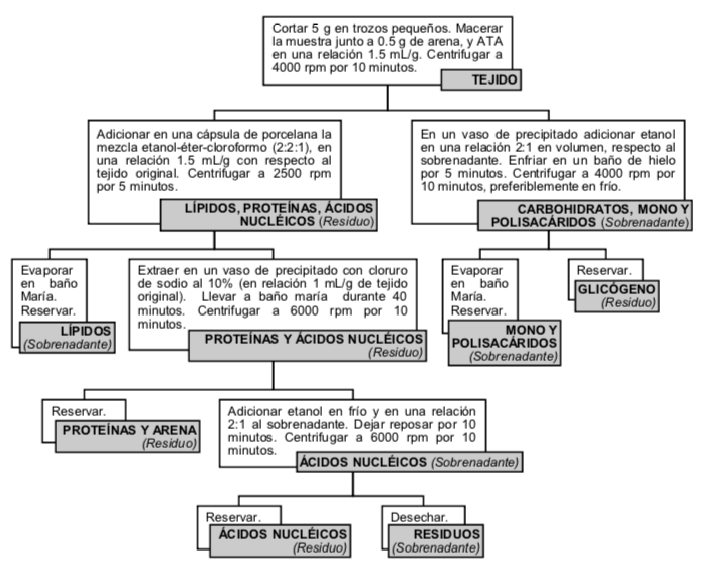
\includegraphics[width = 0.7\linewidth]{fraccionamiento.png}
		\caption{Procedimiento realizado para el fraccionamiento del tejido.}
		\label{fig: fraccionamiento}
	\end{figure*}

	El segundo de estos métodos desarrollados a principios del siglo XX fue la prueba de Molisch, cuyo principio básico fue investigado por Van Ekestein y Blanksma en 1909 \cite{van1910omega}. La prueba requiere de la formación de furfural o 5-hidroximetilfurfural a partir de pentosas y hexosas respectivamente, las cuales se unen a moléculas de $\alpha$-naftol presentes en el reactivo para formar un compuesto con coloración morada \cite{devor1950carbohydrate}. 
	
	El último de estos métodos de análisis de componentes biológicos de muestras biológicas es la prueba con Ninhidrina, cuyo reactivo principal fue descubierto por el químico alemán Siegfried Ruhemann en 1910 \cite{ruhemann1910cxxxii, ruhemann1910ccxii}. La ninhidrina reacciona con el grupo amino de los aminoácidos para formar un producto de coloración morada, el cual es conocido como morado de Ruhemann. Puede ser usado tanto cualitativamente como cuantitativamente, siendo la ninhidrina utilizada para detectar glifosatos con espectroscopía Raman \cite{xu2018indirect}, para realizar secuenciación de péptidos \cite{friedman2004applications} y para determinar el sexo de una persona a partir de residuos encontrados en huellas dactilares \cite{brunelle2016new}. 
	
	Todos estos métodos varían en términos de especificidad y precisión, pero todos son útiles a la hora de determinar la presencia de los diversos compuestos que se desean encontrar en diferentes tejidos humanos y animales, por lo que el objetivo del presente es demostrar la presencia de diversas clases de carbohidratos, lípidos y proteínas en muestras biológicas y compararlas en función de su composición. 

\section{Secci\'on experimental}
	\subsection{Preparación de las soluciones}
		Se prepararon las soluciones como se describe a continuación:
		\begin{enumerate}
			\item \textbf{Ácido clorhídrico al 10 \% v/v:} Se tomaron 2.7 mL de ácido clorhídrico concentrado (37 \%) y se llevó a 10 mL con agua.
			\item \textbf{Hidróxido de sodio al 15 \% p/v:} Se tomaron 1.5 g de hidróxido de sodio y se llevó a 10 mL con agua.
			\item \textbf{Reactivo de Benedict:} Se pesaron 0.18 g de sulfato de cobre (II) pentahidratado, 0.5 g de carbonato de sodio y 0.85 g de citrato de sodio, y se llevó a 10 mL de agua. Agite bien.
			\item \textbf{Reactivo de Biuret:} Se disolvieron 15 mg de sulfato de cobre (II) pentahidratado y 60 mg de tartrato de sodio y potasio tetrahidratado, en 5 mL de agua. Se añadió luego 2 mL de la solución de hidróxido de sodio al 15 \% preparada anteriormente. Posteriormente se adicionó 10 mg de yoduro de potasio. Finalmente se llevó a 10 mL con agua. El reactivo fue almacenado en una botella ámbar pequeña.
			\item \textbf{Reactivo de Molisch:} Se disolvieron 0.1 g de $\alpha$-Naftol en 1 mL de etanol absoluto.
			\item \textbf{Lugol:} Se disolvieron 18 mg de yodo sólido en polvo y 32 mg de yoduro de potasio en polvo en 5 mL de agua. Se agitó vigorosamente hasta la disolución completa de los reactivos. Se cubrió el beaker con papel aluminio.
			\item \textbf{Nihidrina al 0.2 \%:} Se disolvieron 10 mg de ninhidrina en 5 mL de etanol absoluto.
			\item \textbf{Cloruro de sodio al 10 \%:} Se tomó 1 g de cloruro de sodio y se llevó a 10 mL con agua.
			\item \textbf{Éter-Etanol-Cloroformo (2:2:1):} Se Mezclaron 4 mL de éter etílico, 4 mL de etanol absoluto y 2
			mL de cloroformo.
			\item \textbf{Ácido tricloroacético al 10 \%:} Se pesó 1 g de ácido tricloroacético y se llevó a 10 mL con agua.
		\end{enumerate}
	\subsection{Fraccionamiento del tejido}
		
		Se realizó el fraccionamiento de los órganos por grupos independientes siguiendo la \autoref{fig: fraccionamiento}. Los órganos estudiados de manera independiente por los grupos de laboratorio, incluyen: hígado de res, cerebro de res, hígado de pollo y corazón de pollo.
		
	\subsection{Pruebas de identificación}
		Con las muestras obtenidas se realizaron las siguientes pruebas de identificación:
		\subsubsection{Análisis de carbohidratos}
			La muestra se dividió en cuatro fracciones:
			\begin{enumerate}
				\item A la primera se le agregaron 3 gotas de Lugol y se observó el cambio de coloración de la muestra.
				\item A la segunda se le adicionó 1 mL de la solución de ácido clorhídrico al 10 \% y se colocó al baño María por 25 minutos. Se dejó enfriar y se agregaron 3 gotas de Lugol, se observó el cambio de coloración de la muestra.
				\item A la tercera se le adicionó 1 mL de agua destilada y 3 gotas del reactivo de Molisch. Luego se agregó 1 mL de ácido sulfúrico concentrado sin mezclar las dos fases formadas. Se observó la coloración de la muestra.
				\item Se ubicó la cuarta fracción al baño María por 2 minutos, luego se adicionaron 2 mL del reactivo de Benedict. Se observó la coloración en ese momento y 10 minutos después de dejarse en calentamiento. 
			\end{enumerate}
		\subsubsection{Análisis de lípidos}
			La muestra se dividió en 2 fracciones:
			\begin{enumerate}
				\item A la primera se le adicionó 3 mL de cloroformo y se mezcló. Luego se adicionó 1 mL de anhídrido acético. Tras esto se agregaron 3 gotas de ácido sulfúrico. Se observó la coloración de la interfase tras 1 minuto, y después de 15 minutos.
				\item A la segunda se le agregaron 3 mL de hidróxido de sodio al 15 \%. Luego se ubicó al baño maría durante 20 minutos. Finalmente se adicionaron 3 mL de agua destilada y se agitó fuertemente. 
			\end{enumerate}
		
		\subsubsection{Análisis de proteínas}
			La muestra se dividió en 2 fracciones:
			\begin{enumerate}
				\item A la primera se le adicionó 1 mL de agua destilada y se suspendió la muestra. Se agregó 1 mL del reactivo de Biuret y se observó el cambio de coloración.
				\item A la segunda se le agregó 1 mL de la solución de ninhidrina y se calentó al baño María por 10 minutos.
			\end{enumerate}

\section{Resultados y Discusi\'on}

\section{Conclusiones}


%----------------------------------------------------------------------------------------
%	REFERENCE LIST
%----------------------------------------------------------------------------------------
\phantomsection
\bibliography{informe}
\bibliographystyle{unsrt}

%----------------------------------------------------------------------------------------
%\newpage
%\onecolumn
%\section{Informaci\'on suplementaria}\label{sec: complementaria}
\end{document}